



\chapter{Einleitung}

\begin{center}
\begin{figure}[h]
    
\includegraphics[width=\textwidth]{img/PIA23645_PaleBlueDotRevisited_1600.jpg}
    \caption{``The Pale Blue Dot'' Feb. 14, 1990, by NASA\footnotemark.}
    \label{fig:my_label}
\end{figure}
\footnotetext{\fullcite{nasa.bluedot}}
\end{center}

''Ein Bild sagt mehr aus als tausend Worte.`` Dieses bekannte Sprichwort drückt aus, wie mächtig Bilder als Kommunikationsmittel sind. Bilder beinhalten Informationen. Bilder vermitteln Emotionen. Bilder erzählen Geschichten. Bilder sind ein Fenster in die Vergangenheit. Sie sind in der modernen Gesellschaft omnipräsent und wir begegnen sie ständig im Alltag: analog als auch digital.

Bilder sind nicht alle gleich. Sie unterscheiden sich je nach Aufnahme, ihrer digitalen Speicherung oder Darstellung in verschiedenen Eigenschaften. Zwei dieser Eigenschaften sind die Größe und die Auflösung eines Bildes. Die Größe eines digitalen Bildes gibt an, wie viele Pixel es enthält, während die Auflösung eines Bildes angibt, wie viele Pixel pro Flächeneinheit vorhanden sind (PPI). Die Größe und die Auflösung eines Bildes haben Einfluss auf seine Qualität und seinen Speicherplatzbedarf. Um ein Bild für einen bestimmten Zweck zu nutzen, muss man es manchmal in seiner Größe oder Auflösung verändern. Dieser Vorgang wird als Bildskalierung bezeichnet\footfullcite{techlib.scaling}\footfullcite{abcdef.scaling} und ist eine grundlegende Operation in der digitalen Bildverarbeitung.

Bildskalierung ist eine grundlegende Methode der Bildverarbeitung, die es erlaubt, die Größe eines digitalen Bildes zu ändern, ohne seine Qualität zu verschlechtern. Man kann sich das wie eine Zeichnung vorstellen, die man von einem kleinen Papier auf eine große Leinwand überträgt. Wenn man die Zeichnung einfach vergrößert, wird sie unscharf und verliert an Details. Mit der Bildskalierung kann man jedoch dafür sorgen, dass das Bild scharf und detailreich bleibt, egal ob es größer oder kleiner wird.

Es gibt viele verschiedene Methoden, um die Größe eines Bildes zu ändern: Klassische Methoden verwenden Interpolationstechniken, die neue Pixel aus den vorhandenen Pixeln berechnen. Diese Methoden sind schnell und einfach, aber sie können die Qualität des Bildes verschlechtern oder Artefakte erzeugen. Moderne Methoden verwenden Deep-Learning-Techniken wie Convolutional Neural Networks (CNNs) oder Generative Adversarial Networks (GANs), die neue Pixel aus einem trainierten Modell erzeugen. Diese Methoden sind langsam und komplex, aber sie können die Qualität des Bildes verbessern oder kreative Effekte erzielen.

\begin{figure}[h]
    \vspace{8mm}
    \centering
    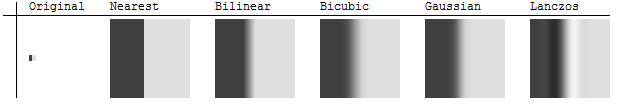
\includegraphics{img/xaR8r.png}
    \caption{Verschiedene Beispiele von upscaling Algorithmen\cite{whuber.lanczos}.}
    \label{fig:my_label}
    \vspace{4mm}
\end{figure}

Die Bildskalierung ist eine wichtige Methode der Bildverarbeitung, die es erlaubt, die Größe und Auflösung von digitalen Bildern zu ändern. Die Bildskalierung hat viele Anwendungen in verschiedenen Bereichen wie Webdesign, Fotografie, Druck oder Videotechnik. Es gibt verschiedene Arten von Skalierungsverfahren, die sich in ihrer Funktionsweise und ihrem Ergebnis unterscheiden. In dieser Arbeit werden wir einen Überblick über die klassischen und modernen Skalierungsverfahren geben und ihre Vor- und Nachteile anhand von Beispielen zeigen. Wir werden auch eine Empfehlung für die beste Skalierungsmethode für verschiedene Bildtypen geben.

In dieser Arbeit geht es darum herauszufinden, welche Methode zum Vergrößern oder Verkleinern von Bildern am besten passt und warum. Dazu erklären wir zuerst die wichtigsten Konzepte der digitalen Bildverarbeitung und der Skalierung von Bildern und zeigen einige Beispiele für ihre Anwendung. Danach stellen wir die traditionellen Skalierungsmethoden vor und vergleichen ihre Stärken und Schwächen. Dann zeigen wir die neueren Skalierungsmethoden und vergleichen ihre Stärken und Schwächen. Zum Schluss bewerten wir die verschiedenen Methoden mit verschiedenen Maßstäben für die Bildqualität und geben eine Empfehlung für die beste Methode. Wir fassen unsere Ergebnisse zusammen und besprechen ihre Bedeutung und Einschränkungen.
